%&../settings/preamble.main

\ifsubfile
\usepackage{../settings/subfile}
\setcounter{chapter}{4}

\usepackage[newfloat, cachedir=_minted-cache, outputdir=../build]{minted}
\usepackage{../libraries/set-minted}

% \usepackage{debug}
\usepackage{transparent}

% arara: pdflatex: { options: ["--output-directory=../build"], shell: yes, draft: yes, synctex: no }
% arara: pdflatex: { options: ["--output-directory=../build"], shell: yes, synctex: no }
\begin{document}
\fi
\chapter{Analisi ammortizzata}

\section{Introduzione}

L'analisi ammortizzata è una tecnica di analisi di complessità che valuta il tempo richiesto per eseguire, nel caso pessimo, una sequenza di operazioni su una struttura dati.
Esistono operazioni più o meno costose.
Se le operazioni più costose sono poco frequenti, allora il loro costo può essere ammortizzato dalle operazioni meno costose.

C'è da notare un'importante differenza.
L'analisi del caso medio è probabilista ed avviene su una singola operazione; mentre l'analisi ammortizzata è deterministica, avviene su operazioni multiple e valuta il caso pessimo.

\subsection{Metodi per l'analisi ammortizzata}

Esistono tre metodi per l'analisi ammortizzata:
\begin{itemize}
    \item metodo dell'\textbf{aggregazione}: si calcola la complessità \(T(n)\) per eseguire \(n\) operazioni in sequenza nel caso pessimo, è una tecnica derivata dalla matematica;
    \item metodo degli \textbf{accantonamenti}: alle operazioni vengono assegnati costi ammortizzati che possono essere maggiori o minori del loro costo effettivo, è un tecnica derivata dall'economia;
    \item metodo del \textbf{potenziale}: lo stato del sistema viene descritto con una funzione di potenziale, è una tecnica derivata dalla fisica.
\end{itemize}

\section{Contatore binario}

\paragraph{Descrizione del problema}
Prendiamo in considerazione un contatore binario di \(k\) bit con un vettore \(A\) di booleani 0/1.
Dove il bit meno significativo si trova in \(A[0]\), e il bit più significatico \(A[k-1]\).
L'operazione di \increment{} incrementa il contatore di una unità.
Il valore del contatore è:
\[
    x = \sum_{i=0}^{k-1} A[i] \, 2^i
\]

L'\cref{alg:contatore-binario} illustra i passaggi\dots

\begin{algorithm}[hb]
    \caption{Incremento di un contatore binario}%
    \label{alg:contatore-binario}
    \prototype{\Int \increment{\Array{\Int}[] \(A\), \Int \(k\)}}{
        
        \BlankLine
        \Int \(i\) \Assign \(0\)\;
        
        \BlankLine
        \While{\(i < k\) \And \(A[i] \Equal 1\) }{
            \(A[i]\) \Assign 0\;
            \Increment{i}\; 
        }
        
        \BlankLine
        \If{\(i < k\)}{
            \(A[i]\) \Assign \(1\)\;
        }
    }
\end{algorithm}

Nella~\cref{tab:contatore-bit} notiamo che i bit modificati\dots

\begin{table}[!ht]\centering
    \caption{Esempio di contatore binario}%
    \label{tab:contatore-bit}
    \begin{tabular}{@{} *{9}{ F{C} } @{}}
        \toprule
            x & A[7] & A[6] & A[5] & A[4] & A[3] & A[2] & A[1] & A[0]\\
        \midrule
            0 & & & & & & & & \\
        \lightrule
            1 & & & & & & & & \textbf{1}\\
        \lightrule
            2 & & & & & & & \textbf{1} & \\
        \lightrule
            3 & & & & & & & \textbf{1} & \textbf{1}\\
        \lightrule
            4 & & & & & & \textbf{1} & & \\
        \lightrule
            5 & & & & & & \textbf{1} & & \textbf{1}\\
        \lightrule
            6 & & & & & & \textbf{1} & \textbf{1} & \\
        \lightrule
            7 & & & & & & \textbf{1} & \textbf{1} & \textbf{1}\\
        \lightrule
            8 & & & & & \textbf{1} & & & \\
        \lightrule
            9 & & & & & \textbf{1} & & & \textbf{1}\\
        \lightrule
            10 & & & & & \textbf{1} & & \textbf{1} & \\
        \lightrule
            11 & & & & & \textbf{1} & & \textbf{1} & \textbf{1}\\
        \lightrule
            12 & & & & & \textbf{1} & \textbf{1} & & \\
        \lightrule
            13 & & & & & \textbf{1} & \textbf{1} & & \textbf{1}\\
        \lightrule
            14 & & & & & \textbf{1} & \textbf{1} & \textbf{1} & \\
        \lightrule
            15 & & & & & \textbf{1} & \textbf{1} & \textbf{1} & \textbf{1}\\
        \lightrule
            16 & & & & \textbf{1} & & & & \\
        \bottomrule
    \end{tabular}
\end{table}

\subsection{Metodo dell'aggregazione}

Nel metodo dell'aggregazione si calcola la complessità \(T(n)\) per eseguire \(n\) operazioni in sequenza nel caso pessimo.
Si calcola poi il costo ammortizzato \(T(n)/n\) come media su \(n\) operazioni.

Si considera l'evoluzione della struttura dati data la peggior sequenza di operazioni.
Si effettua la sommatoria delle complessità individuali, per questo si chiama metodo dell'aggregazione.

Qual è il costo \(T(n)\) per eseguire \(n\) operazioni (nel caso pessimo)?
Qual è il costo ammortizzato \(T(n)/n\)?

Facciamo un'analisi \enquote{grossolana}.
Sono necessari \(k = \ceil{\log(n+1)}\) bit per rappresentare \(n\).
Una chiamata \increment{} richiede tempo \(\Omicron(k)\) nel caso pessimo.
Il costo di \(n\) operazioni è \(T(n) = \Omicron(nk)\), il costo di un'operazione si può calcolare semplicemente dividendo per le \(n\) operazioni, \(T(n)/n = \Omicron(k) = \Omicron(\log n)\).

Il grafico mostrato il costo ammortizzato di un'operazione con \(n = 2^k\) operazioni (\(k \in [20, 35]\)).
Eseguito in Java.

\begin{figure}[!ht]\centering
    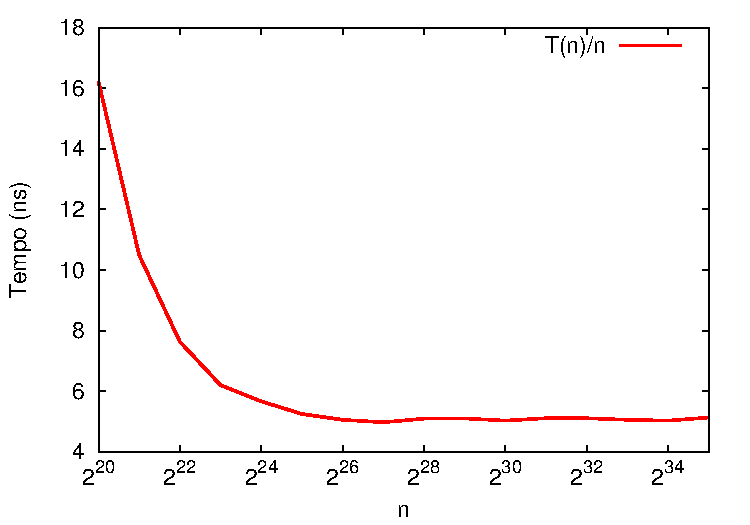
\includegraphics[width=.65\textwidth]{ops-ammortizzate}
    \caption{Didascalia}\label{fig:ops-ammortizzate}
\end{figure}

\subsubsection{Metodo dell'aggregazione nel contatore binario}

Possiamo osservare che il tempo necessario ad eseguire l'intera sequenza è proporzionale al numero di bit che vengono modificati.
Quanti bit vengono modificati?

\newcommand{\diff}[1]{\textcolor{red}{\textbf{#1}}}

\begin{table}[!ht]\centering
    \caption{Numero di bit modificati}%
    \label{tab:contatore-bit-modificati}
    \begin{tabular}{@{} *{9}{ F{C} } C @{}}
        \toprule
            x & A[7] & A[6] & A[5] & A[4] & A[3] & A[2] & A[1] & A[0] & \texttt{\#}\text{bit}\\
        \midrule
            0 & & & & & & & & \\
        \lightrule
            1 & & & & & & & & \diff{1} & 1\\
        \lightrule
            2 & & & & & & & \diff{1} & \diff{0} & 2\\
        \lightrule
            3 & & & & & & & \textbf{1} & \diff{1} & 1\\
        \lightrule
            4 & & & & & & \diff{1} & \diff{0} & \diff{0} & 3\\
        \lightrule
            5 & & & & & & \textbf{1} & \textbf{0} & \diff{1} & 1\\
        \lightrule
            6 & & & & & & \textbf{1} & \diff{1} & \diff{0} & 2\\
        \lightrule
            7 & & & & & & \textbf{1} & \textbf{1} & \diff{1} & 1\\
        \lightrule
            8 & & & & & \diff{1} & \diff{0} & \diff{0} & \diff{0} & 4\\
        \lightrule
            9 & & & & & \textbf{1} & \textbf{0} & \textbf{0} & \diff{1} & 1\\
        \lightrule
            10 & & & & & \textbf{1} & \textbf{0} & \diff{1} & \diff{0} & 2\\
        \lightrule
            11 & & & & & \textbf{1} & \textbf{0} & \textbf{1} & \diff{1} & 1\\
        \lightrule
            12 & & & & & \textbf{1} & \diff{1} & \diff{0} & \diff{0} & 3\\
        \lightrule
            13 & & & & & \diff{1} & \diff{1} & \diff{0} & \diff{1} & 1\\
        \lightrule
            14 & & & & & \textbf{1} & \textbf{1} & \diff{1} & \diff{0} & 2\\
        \lightrule
            15 & & & & & \textbf{1} & \textbf{1} & \textbf{1} & \diff{1} & 1\\
        \lightrule
            16 & & & & \diff{1} & \diff{0} & \diff{0} & \diff{0} & \diff{0} & 5\\
        \midrule
            \texttt{\#}\text{bit} & 0 & 0 & 0 & 1 & 2 & 4 & 8 & 16\\
        \bottomrule
    \end{tabular}
\end{table}

Dalla~\cref{tab:contatore-bit-modificati} si può notare che \(A[0]\) viene modificato ogni incremento, \(A[1]\) ogni due incrementi, \(A[2]\) ogni quattro incrementi\dots \(A[i]\) ogni \(2^i\) incrementi.

Il costo totale risultante risulta:
\[\begin{WithArrows}[displaystyle]
T(n) &= \sum_{i=0}^{k-1} \floor*{\frac{n}{2^i}} \Arrow{porto fuori \(n\)}\\
     &\leqslant n \sum_{i=0}^{k-1} \floor*{\frac{1}{2^i}} \Arrow{estendo la sommatoria}\\
     &\leqslant n \sum_{+\infty}^{k-1} \braces*{\frac{n}{2^i}}^i \Arrow{semplifico la sommatoria}\\
     &= 2n
\end{WithArrows}\]
Il costo ammortizzato è \(T(n)/n \leqslant 2n/n = 2 = \Omicron(1)\).

\subsection{Metodo degli accantonamenti}

Nel metodo degli accantonamenti si assegna un costo ammortizzato \emph{potenzialmente} distinto ad ognuna delle operazioni possibili.
Il costo ammortizzato può essere diverso dal costo effettivo.
Le operazioni meno costose vengono caricate di un costo aggiuntivo detto credito.
\[
    \text{costo ammortizzato} = \text{costo effettivo} + \text{credito prodotto}
\]
I crediti accumulati sono usati per pagare le operazioni più costose
\[
    \text{costo ammortizzato} = \text{costo effettivo} - \text{credito consumato}
\]

\subsubsection{Obiettivi}

Ci fissiamo due obiettivi.
\begin{enumerate}
    \item Dimostrare che la domma dei costi ammortizzati \(a_i\) è un limite superiore ai costi effettivi \(c_i\):
    \[
        \sum_{i=1}^{n} c_i \leqslant \sum_{i=1}^{n} a_i
    \]
    \item dimostrare che il valore così ottenuto è \enquote{poco costoso}.
\end{enumerate}

Quando cerchiamo di dimostrare quanto sopra, dobbiamo ricordare alcuni punti importanti:
\begin{itemize}
    \item la dimostrazione deve per tutte le sequenze (anche nel caso pessimo);
    \item il credito dopo l'operazione \(t\)-esima è espresso dalla seguente formula ed è sempre positivo:
    \[
        \sum_{i=1}^{t} a_i - \sum_{i=1}^{t} c_i \geqslant 0
    \]
\end{itemize}

\subsubsection{Metodo degli accantonamenti nel contatore binario}

% \begin{proof}[Metodo degli accantonamenti per il contatore binario]
Il costo dell'operazione \increment{} è \(d\), dove \(d\)  è il numero di bit che cambiano valore;
il costo ammortizzato dell'operazione \increment{} è \(2\): \(1\) per il cambio di un bit da \(0\) a \(1\) (il costo effettivo) e \(1\) per il futuro cambio dello stesso bit da \(1\) a \(0\).
Ne consegue che in ogni istante, il credito è pari al numero di bit \(1\) presenti.

Il costo totale risultante è \(\Omicron(n)\), il costo ammortizzato \(\Omicron(1)\).
% \end{proof}

\subsection{Metodo del potenziale}

\begin{definition*}[Funzione di potenziale]
Una funzione di potenziale \(\Phi\) associa ad uno stato \(S\) della struttura dati la \enquote{quantità di lavoro} \(\Phi(S)\) che è stato contabilizzato nell'analisi ammortizzata, ma non ancora eseguito. 
\end{definition*}

In altre parole, \(\Phi(S)\) rappresenta la quantità di energia potenziale \enquote{immagazzinata} in quello stato.

Il costo ammortizzato viene così definitivo come
\[
    \text{costo ammortizzato} = \text{costo effettivo} + \text{variazione di potenziale}    
\]
ossia
\[
    a_i = c_i + \Phi(S_i) - \Phi(S_{i-1})
\]
dove \(S_i\) è lo stato associato alla \(i\)-esima operazione.

\subsubsection{Costo ammortizzato}

Il costo ammortizzato di calcola su una sequenza di \(n\) operazioni.
\[\begin{WithArrows}[displaystyle]
A &= \sum_{i=1}^{n} a_i \Arrow{sostituisco \(a_i\)}\\
  &= \sum_{i=1}^{n} c_i + \Phi(S_i) - \Phi(S_{i-1}) \Arrow{divido la sommatoria}\\
  &= \sum_{i=1}^{n} c_i + \sum_{i=1}^{n} (\Phi(S_i) - \Phi(S_{i-1})) \Arrow{svolgo le sommatorie}\\
  &= C + \Phi(S_1) - \Phi(S_0) + \Phi(S_2) - \Phi(S_1) + \cdots + \Phi(S_n) - \Phi(S_{n-1}) \Arrow{semplifico}\\
  &= C + \Phi(S_n) - \Phi(S_0)
\end{WithArrows}\]

Se la variazione di potenziale \(\Phi(S_n) - \Phi(S_0)\) è non negativa, il costo ammortizzato \(A\) è un limite superiore al costo reale.

\subsubsection{Metodo del potenziale nel contatore binario}

Riprendendo l'esempio del contatore binario prendiamo come funzione potenziale \(\Phi\) il numero di bit \(1\) presenti nel contatore.
Nell'operazione \increment{} \(t\) è il numero di bit \(1\) incontrati a partire dal meno significatico, prima di incontrare un bit \(0\).
Il costo effettivo risultato \(1+t\), la variazione di potenziale \(1-t\) ed il costo ammortizzato \(1+t + 1-t = 2\).

All'inizio ci sono zero bit accesi quindi \(\Phi(S_0) = 0\), mentre alla fine \(\Phi(S_0) \geqslant 0\), la differenza di potenziale è non negativa, quindi siamo certi che il costo ammortizzato sia un limite superiore al costo reale.

\section{Vettori dinamici}

Nelle sequenze implementate come vettori dinamici si alloca un vettore di una certa dimensione detta capacità.
L'inserimento di un elemento \enquote{in mezzo} ha costo \(\Omicron(n)\) (\cref{fig:vector-insert}).
Inserire un elemento \enquote{in fondo} alla sequenza (operazione di \texttt{append}) ha costo \(\Omega(1)\) (\cref{fig:vector-append}).

\begin{figure}[!ht]
    \hfill
    \begin{subfigure}[b]{.3\linewidth}
        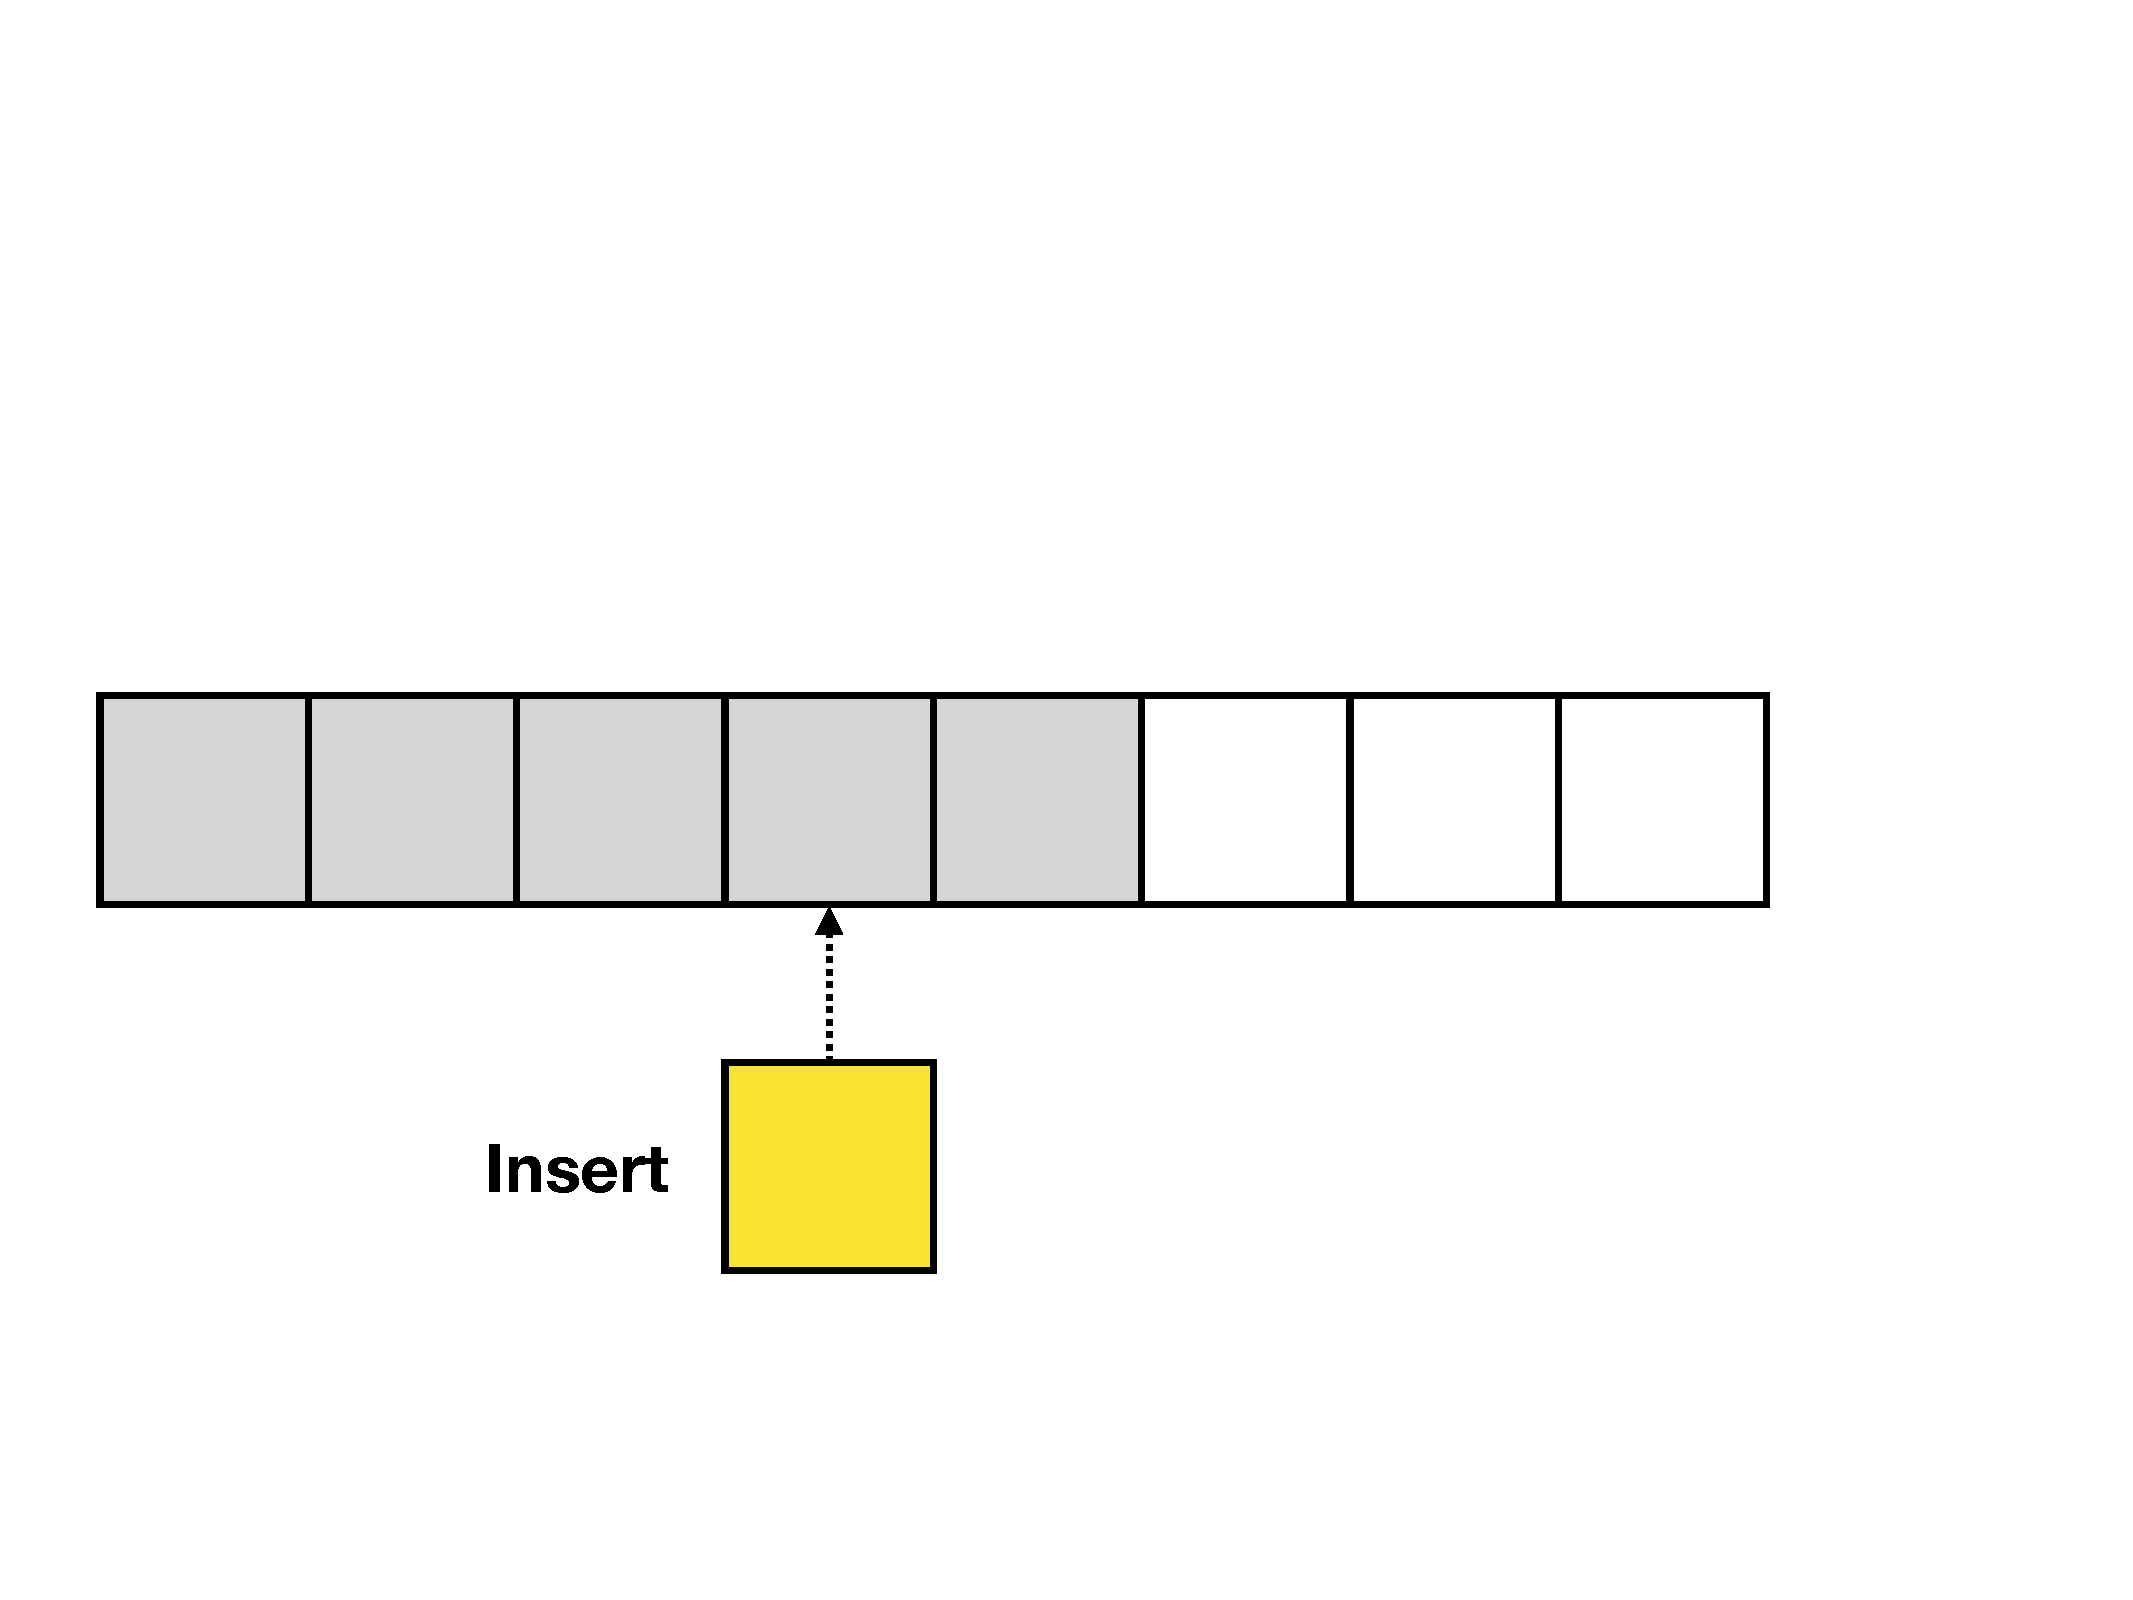
\includegraphics[width=\linewidth, page=1]{vector-insert}
        
        \vspace{5pt}
        \includegraphics[width=\linewidth, page=2]{vector-insert}

        \vspace{5pt}
        \includegraphics[width=\linewidth, page=3, trim=0 180pt 0 40pt, clip]{vector-insert}
        \caption{Inserimento \enquote{in mezzo}}\label{fig:vector-insert}
    \end{subfigure}
    \hfill
    \begin{subfigure}[b]{.3\linewidth}
        \centering
        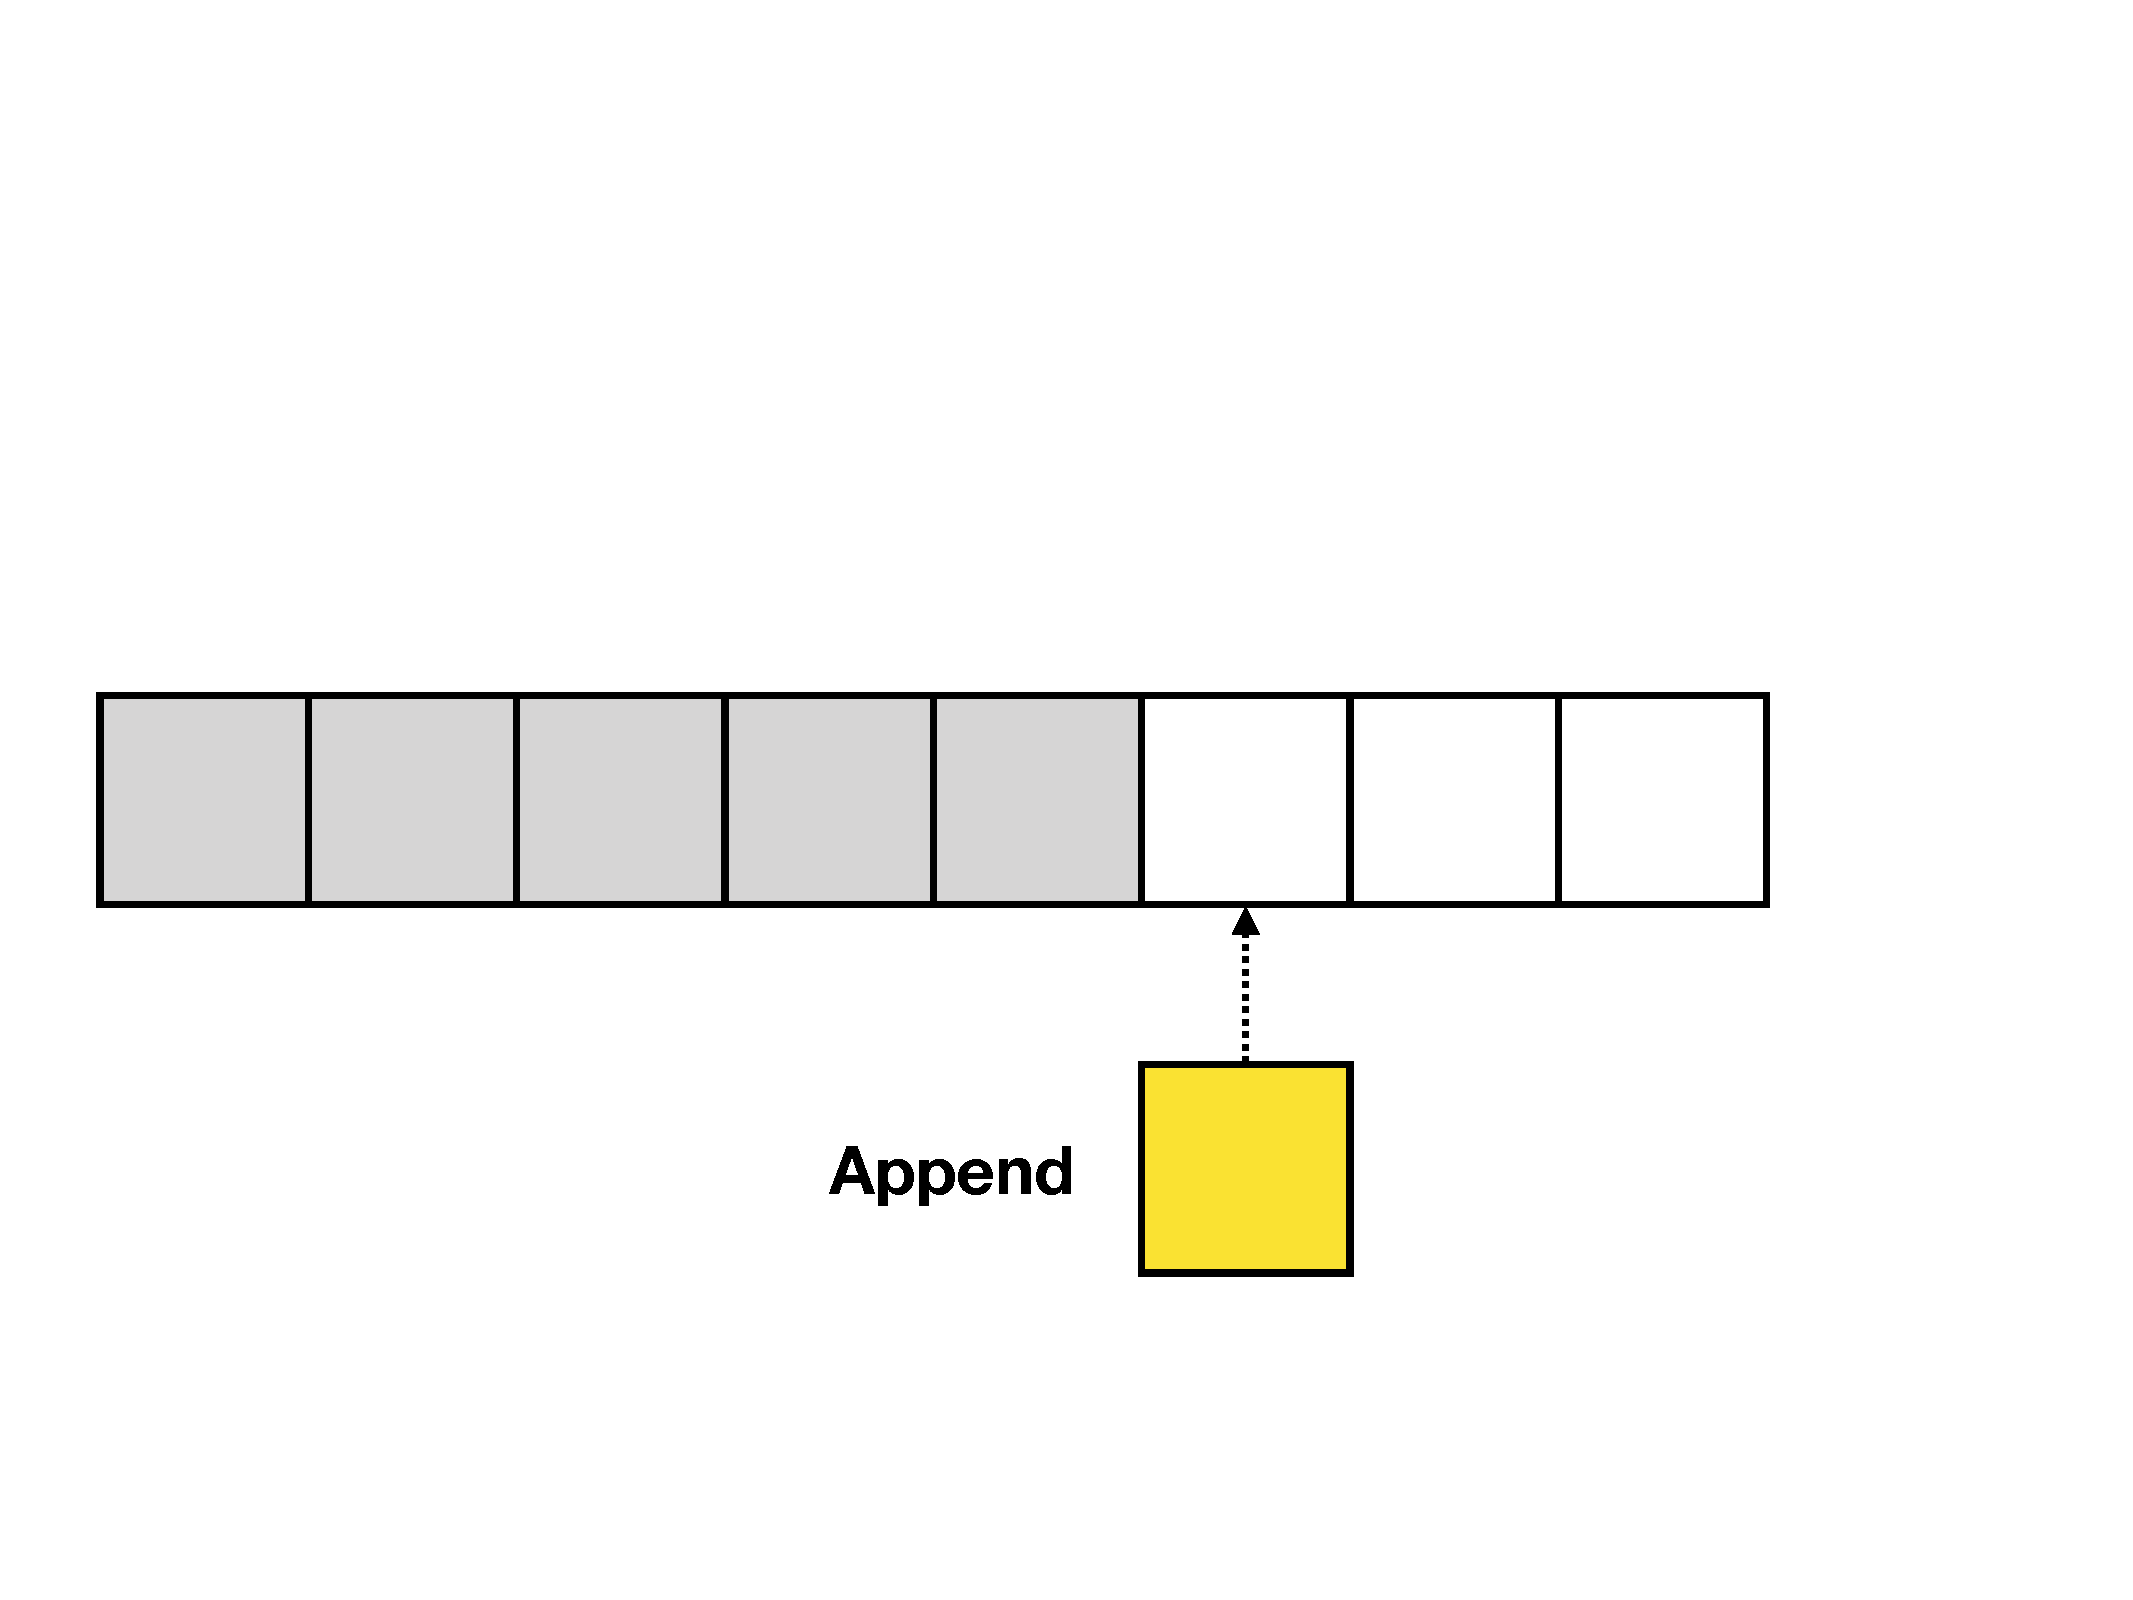
\includegraphics[width=\linewidth, page=1]{vector-append}
        
        \vspace{5pt}
        \includegraphics[width=\linewidth, page=2]{vector-append}

        \caption{Inserimento in coda}\label{fig:vector-append}
    \end{subfigure}
    \hfill
    % TODO richiedere illustazione vector-remove a Montresor
    \begin{subfigure}[b]{.3\linewidth}
        {\transparent{0.2}
        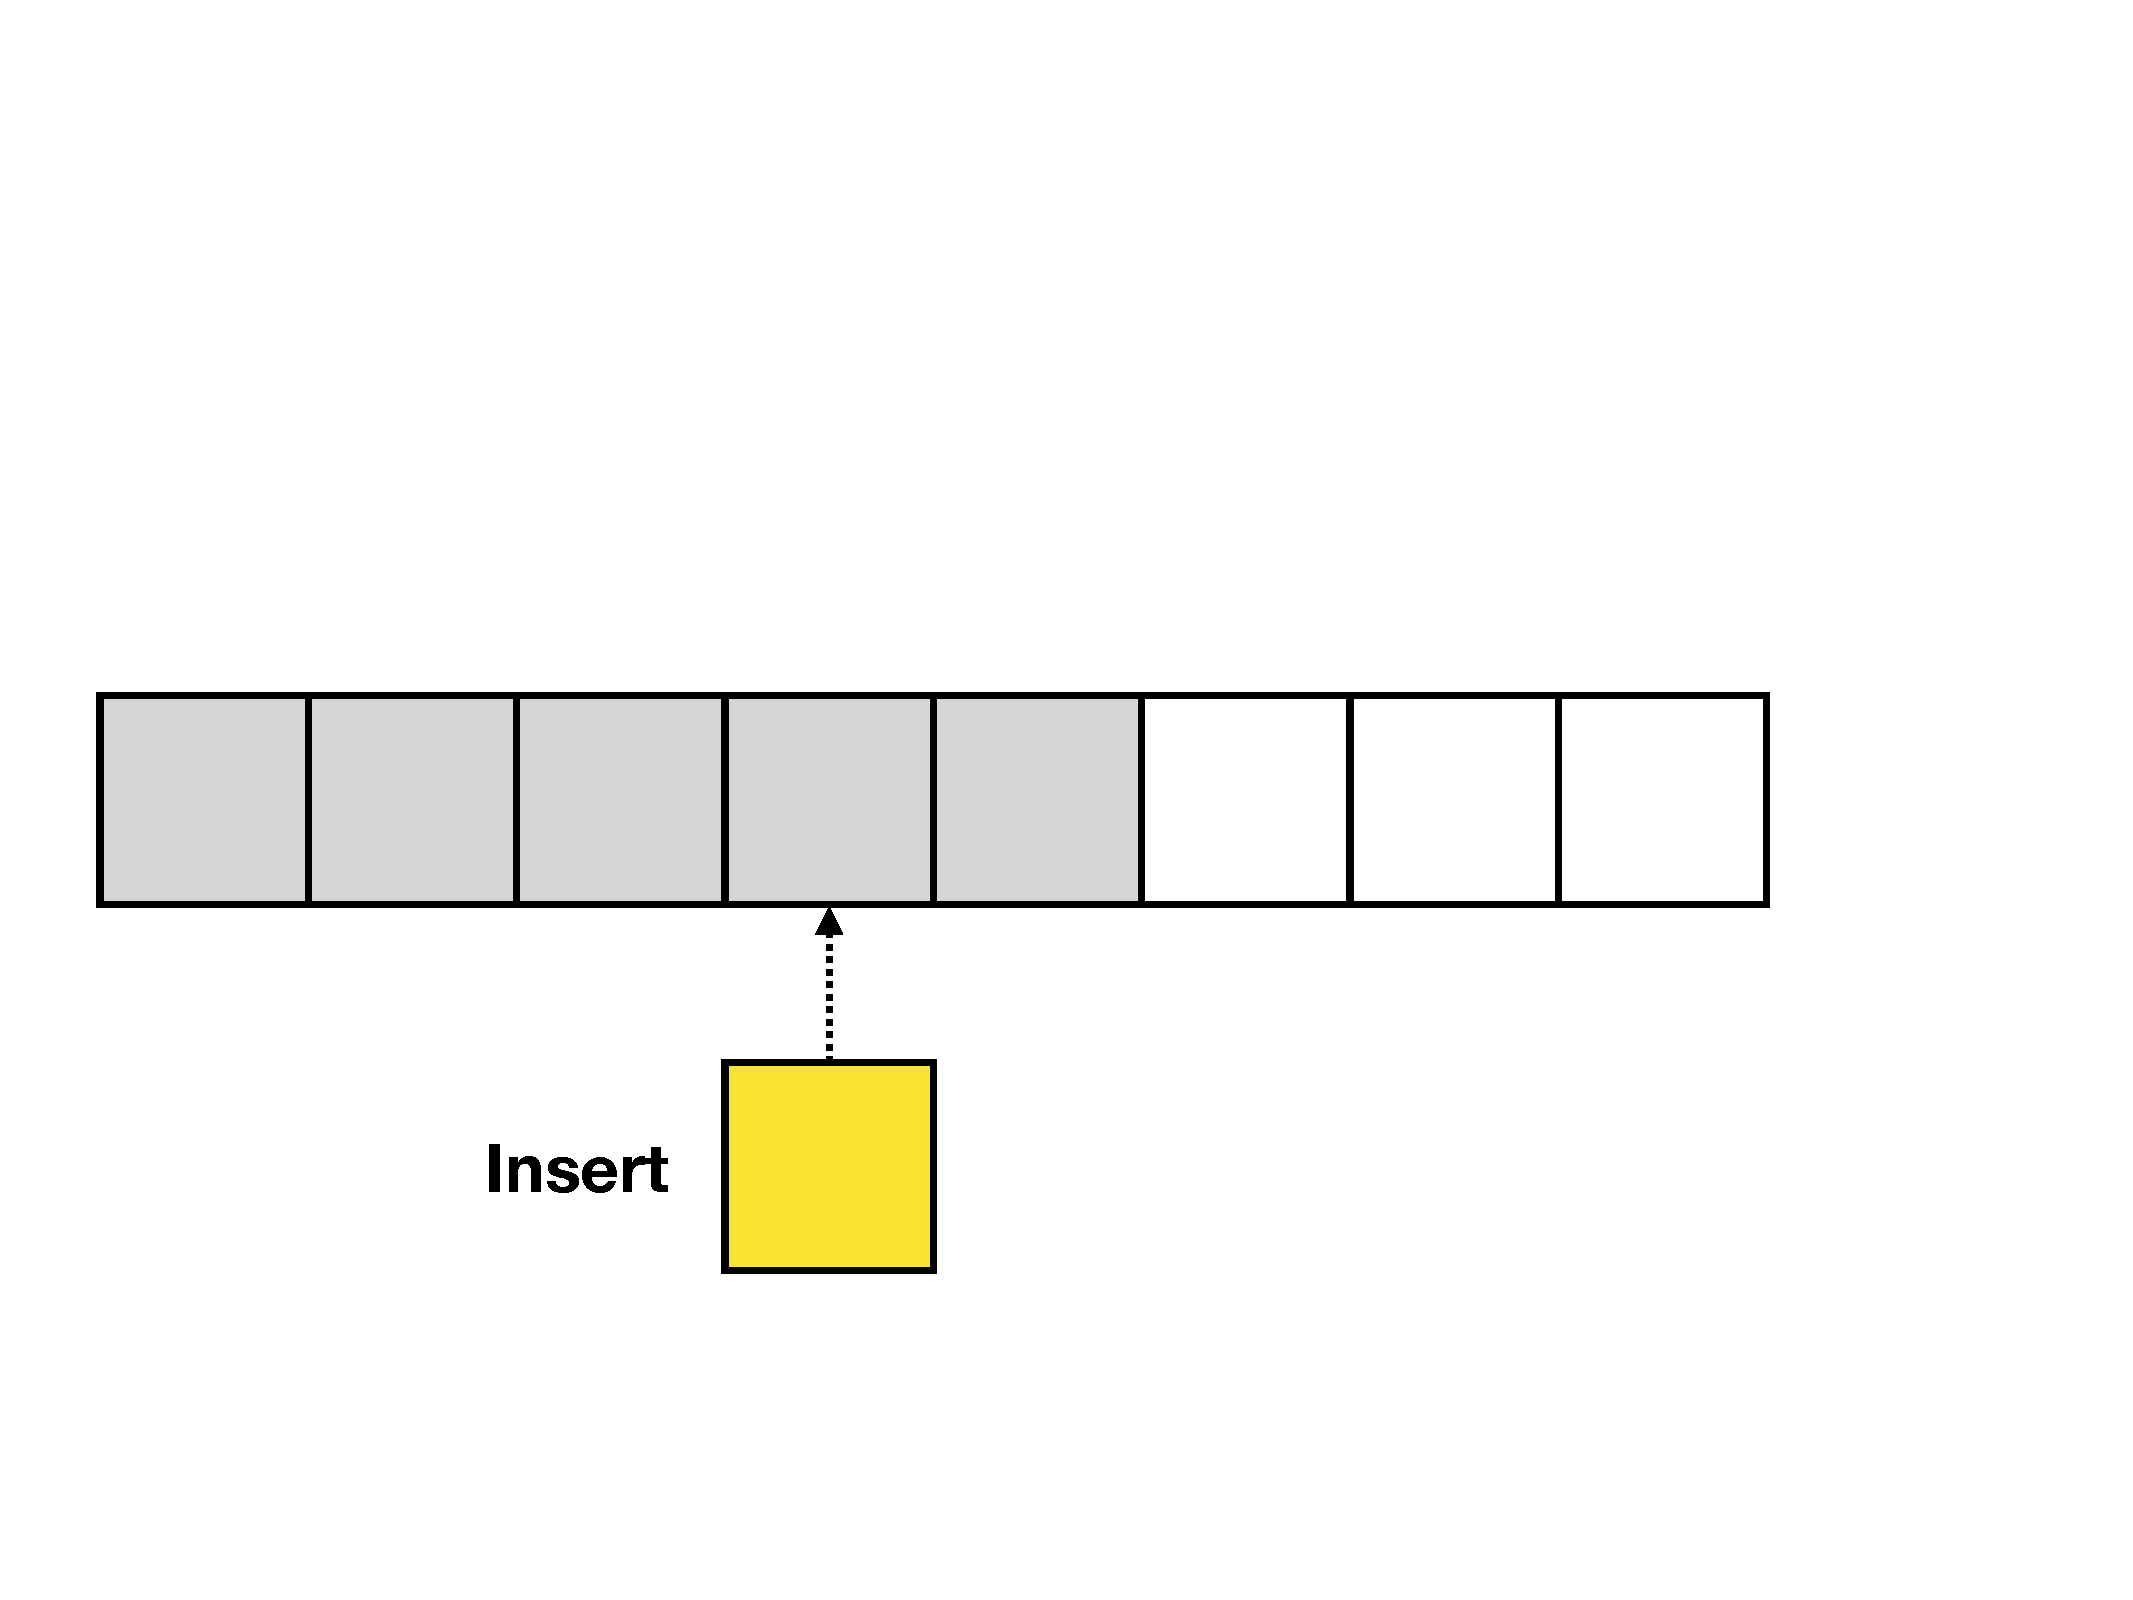
\includegraphics[width=\linewidth, page=1]{vector-insert}
        % \includegraphics[width=\linewidth, page=1]{vector-remove}
        
        \vspace{5pt}
        \includegraphics[width=\linewidth, page=2]{vector-insert}
        % \includegraphics[width=\linewidth, page=2]{vector-remove}

        \vspace{5pt}
        \includegraphics[width=\linewidth, page=3, trim=0 180pt 0 40pt, clip]{vector-insert}}
        % \includegraphics[width=\linewidth, page=3, trim=0 180pt 0 40pt, clip]{vector-remove}
        \caption{Rimozione di un elemento}\label{fig:vector-insert}
    \end{subfigure}
    \hfill\null
    \caption{Operazioni di inserimento \enquote{in mezzo}, inserimento in coda e rimozione di un elemento in un vettore}
\end{figure}

\paragraph{Descrizione del problema}
Non è noto a priori quanti elementi entreranno nella sequenza.
La capacità selezionata può rivelarsi insufficiente.

\paragraph{Soluzione}
Si alloca un vettore di capacità maggiore, si ricopia il contenuto del vecchio vettore nel nuovo e si rilascia il vecchio vettore.

Ne sono esempi le librerie java \texttt{java.util.Vector} e \texttt{java.util.ArrayList}.
Un esempio di implementazione dei vettori dinamici in Java è presentato nel~\cref{lst:vettori-dinamici-java}.

\begin{listing}[H]
\caption{Vettori dinamici in Java}\label{lst:vettori-dinamici-java}
\begin{minted}{java}
private Object[] buffer = new Object[INITSIZE];

// Utilizzato in ArrayList (1.2)
private void doubleStorage() {
    Object[] newb = new Object[2*buffer.length]; // raddoppiamento
    System.arraycopy(buffer,0, newb,0, buffer.length);
    buffer = newb;
}

// Utilizzato in Vector (1.0)
private void incrementStorage() {
    Object[] newb = new Object[buffer.length+INCREMENT]; // incremento fisso
    System.arraycopy(buffer,0, newb,0, buffer.length);
    buffer = newb;
}
\end{minted}
\end{listing}

Dalla documentazione Java di \textsf{ArrayList.add()} possiamo leggere:
\enquote{\foreign{As elements are added to an ArrayList, its capacity grows automatically. The details of the growth policy are not specified beyond the fact that adding an element has constant amortized time cost.}}

Quale strategia è la migliore fra le due?
Il raddoppiamento della dimensione o l'incremento costante?
Effettuiamo l'anlisi ammortizzata di entrambi i casi.

\subsubsection{Analisi ammortizzata del raddoppiamento del vettore}

Assumendo che la dimensione iniziale del vettore sia \(1\) e che il costo di scrittura di un elemento sia \(1\).
Il costo effettivo di un'operazione \textsf{add()} è dato dalla seguente espressione:
\[
    c_i =
    \begin{dcases}
        i & \exists k \in \mathbb{Z}_{0}^{+}\; : i = 2^k + 1\\
        1 & \text{altrimenti}\\
    \end{dcases}
\]

\begin{center}
\captionof{table}{costo effettivo di un'operazione di raddoppiamento di un vettore}
\begin{tabular}{@{} L*{17}{C} @{}}
    \toprule
        n & 1 & 2 & 3 & 4 & 5 & 6 & 7 & 8 & 9 & 10 & 11 & 12 & 13 & 14 & 15 & 16 & 17\\
    \midrule
        \text{costo} & 1 & \textbf{2} & \textbf{3} & 1 & \textbf{5} & 1 & 1 & 1 & \textbf{9} & 1 & 1 & 1 & 1 & 1 & 1 & 1 & \textbf{17}\\
    \bottomrule
\end{tabular}
\end{center}

Scrivere spiegazione\dots

Il costo effettivo di \(n\) operazioni di raddoppiamento sono:
\[\begin{WithArrows}[displaystyle]
T(n) &= \sum_{i=1}^{n} c_i \Arrow{spiegazione}\\
     &= n + \sum_{j=0}^{\floor{\log n}} 2^j \Arrow{spiegazione}\\
     &= n + 2^{\floor{\log n} + 1} - 1 \Arrow{spiegazione}\\
     &\leqslant n + 2^{\log n + 1} - 1 \Arrow{spiegazione}\\
     &\leqslant n + 2n - 1 = \Omicron(n)
\end{WithArrows}\]
Il costo ammortizzato di un'operazione  è quindi \(T(n)/n = \Omicron(n)/n = \Omicron(1)\).

\subsubsection{Analisi ammortizzata dell'incremento del vettore}

Assumendo che la dimensione iniziale del vettore sia \(d\), che il costo di scrittura di un elemento sia \(1\) e che l'incremento sia grande \(d\) (nell'esempio \(d=4\)).
Il costo effettivo di un'operazione \textsf{add()} è dato dalla seguente espressione:
\[
    c_i =
    \begin{dcases}
        i & (i\mod d) = 1\\
        1 & \text{altrimenti}\\
    \end{dcases}
\]

\begin{center}
\captionof{table}{costo effettivo di un'operazione di incremento di un vettore}
\begin{tabular}{@{} L*{17}{C} @{}}
    \toprule
        n & 1 & 2 & 3 & 4 & 5 & 6 & 7 & 8 & 9 & 10 & 11 & 12 & 13 & 14 & 15 & 16 & 17\\
    \midrule
        \text{costo} & 1 & 1 & 1 & 1 & \textbf{5} & 1 & 1 & 1 & \textbf{9} & 1 & 1 & 1 & \textbf{13} & 1 & 1 & 1 & \textbf{17}\\
    \bottomrule
\end{tabular}
\end{center}

Scrivere spiegazione\dots

Il costo effettivo di \(n\) operazioni di incremento sono: 
\[\begin{WithArrows}[displaystyle]
T(n) &= \sum_{i=1}^{n} c_i \Arrow{spiegazione}\\
     &= n + \sum_{j=1}^{\floor{n/d}} d \cdot j \Arrow{spiegazione}\\
     &= n + d \sum_{j=1}^{\floor{n/d}} d \cdot j \Arrow{spiegazione}\\
     &= n + d \frac{(\floor{n/d} + 1) \floor{n/d}}{2} \Arrow{spiegazione}\\
     &\leqslant n + \frac{(n/d + 1) n}{2} = \Omicron(n^2)
\end{WithArrows}\]
Il costo ammortizzato di un'operazione  è quindi \(T(n)/n = \Omicron(n^2)/n = \Omicron(n)\).

\begin{table}[H]\centering
    \caption{Reality check}
    \begin{tabular}{@{} llS @{}}
        \toprule
            \textbf{Linguaggio} & \textbf{Struttura dati} & \textbf{Fattore} \\
        \midrule
            \texttt{GNU C++} & \texttt{std::vector} & 2.0\\
        \lightrule
            \texttt{Microsoft VC++ 2003} & \texttt{vector} & 1.5\\
        \lightrule
            \texttt{C\#} & \texttt{List} & 2.0\\
        \lightrule
            \texttt{Python} & \texttt{list} & 1.125\\
        \lightrule
            \texttt{Oracle Java} & \texttt{ArrayList} & 2.0\\
        \lightrule
            \texttt{OpenSDK Java} & \texttt{ArrayList} & 1.5\\
        \bottomrule
    \end{tabular}
\end{table}

\subsubsection{Allocazione memoria}

Quanto memoria occupa un intero \(32\) bit se memorizzato in un vettore dinamico o in un elemento di una lista, nel caso pessimo/ottimo?

Nel caso ottimo, ossia nel caso in cui un vettore sia pieno, \(4n\) byte;
mentre nel caso pessimo, ossia quello in cui il vettore è appena stato raddoppiato, \(2 \cdot 4n\) byte.

Alcuni dati interessanti (e inquietanti) relativi a Java:
\begin{itemize}
    \item un \textsf{Object} vuoto richiede 16 byte in un’architettura a 64 bit;
    \item l'allocazione di memoria avviene per multipli di 8 byte;
    \item un oggetto contenente un intero e due reference (lista bidirezionale) richiede 32-40 byte (Java compressed references).
\end{itemize}

\begin{listing}[H]
\caption{String vs StringBuffer}
\begin{minted}{java}
public static void print(int dim) {
    StringBuffer buffer = new StringBuffer();
    for (int i=0; i < dim; i++) {
        buffer.append('x');
    }

    String string = new String();
    for (int i=0; i < dim; i++) {
        string = string + 'x';
    }
}
\end{minted}
\end{listing}

\begin{table}[htbp]\centering
    \caption{didascalia}\label{tab:etichetta}
    \begin{tabular}{@{} S[table-format=7] S[table-format=2] S[table-format=6] @{}}
        \toprule
            {\texttt{dim}} & {\texttt{StringBuffer} (ms)} & {String (ms)} \\
        \midrule
               1024 &  0 & 3     \\
               2048 &  1 & 7     \\
               4096 &  1 & 13    \\
               8192 &  1 & 22    \\
              16384 &  3 & 71    \\
              32768 &  4 & 285   \\
              65536 &  3 & 1130  \\
             131072 &  4 & 4847  \\
             262144 &  6 & 20853 \\
             524288 & 11 & 84982 \\
            1048576 & 24 & 400653\\
        \bottomrule
    \end{tabular}
\end{table}

\subsubsection{Somme di stringhe in Python}

\begin{listing}[H]
\caption{Somme di stringhe in Python}
\begin{minted}{java}
s = ""
for i in range(10000):
    s = s + "1"
\end{minted}
\end{listing}

In CPython, questo codice viene ottimizzato utilizando \textsf{realloc}, invece di \textsf{malloc} e ha costo lineare, fino ad un certo punto.
Oltre una certa dimensione, il costo torno ad essere quadratico.
Altre implementazioni di Python non seguono questo approccio.
Per approfondire \href{https://stackoverflow.com/questions/4435169/}{https://stackoverflow.com/questions/4435169/}.

\subsection{Analisi ammortizzata della cancellazione di un elemento del vettore}

Quanto costa togliere un elemento da un vettore e da un vettore non ordinato?

Dobbiamo introdurre il concetto di \emph{contrazione}.
Per ridurre lo spreco di memoria, è opportuno contrarre il vettore quando il fattore di carico \(\alpha = \text{dim}/\text{capacità}\) diventa troppo piccolo, dove la dimensione è il numero di elementi attualmente presenti.

L'operazione di contrazione presuppone che vengano copiati gli elementi e che poi venga deallocata la memoria in eccesso.

A questo punto ci domandiamo: quale soglia utilizzare per il fattore di carico?

\paragraph{Strategia banale}
Una strategia banale (na\"if) è dimezzare la memoria quando il fattore di carico \(\alpha\) diventa \(1/2\).
Dimostriamo che questa strategia può portare ad un costo ammortizzato lineare.

Considerate la seguente sequenza di \textbf{I}nserimenti e \textbf{R}imozioni in un vettore di capacità 8:

\begin{center}
\begin{tabular}{@{} *{14}{>{\ttfamily}l} @{}}
    Ops: I I I I I R I R I R I R I\\
    Dim: 1 2 3 4 5 4 5 4 5 4 5 4 5\\
    Cap: 8 8 8 8 8 4 8 4 8 4 8 4 8\\
\end{tabular}
\end{center}

Qual è il problema?
Non abbiamo un numero di inserimenti/rimozioni sufficienti per ripagare le espansioni/contrazioni
Dobbiamo lasciar decrescere il sistema ad un fattore inferiore a \(1/4\), dopo un'espansione o una contrazione, il fattore di carico diventa \(1/2\).

\subsubsection{Analisi ammortizzata per la contrazione di un vettore}

Usiamo una funzione di potenziale che vale 0 all'inizio e subito dopo un'espansione o contrazione e che cresce fino a raggiungere il numero di elementi presenti nella tavola quando \(\alpha\) aumenta fino ad 1 o diminuisce fino ad \(1/4\). 
\[
    \Phi =
    \begin{dcases}
        2 \cdot \text{dim} - \text{capacità} & \alpha \geqslant \frac{1}{2}\\
        \text{capacità}/2 - \text{dim}       & \alpha \leqslant \frac{1}{2}\\
    \end{dcases}
\]
Prendiamo in considerazione alcuni casi esplicativi:
\begin{itemize}
    \item dopo un'espansione o contrazione \(\alpha=\frac{1}{2}\), la funzione di potenziale \(\Phi=0\);  
    \item prima di un'espansione \(\alpha=1\), la dimensione risulta pari alla capacità e la funzione di potenziale è pari alla dimensione del vettore (\(\Phi=\text{dim}\));
    \item prima di una contrazione \(\alpha=\frac{1}{4}\), la capacità risulta quattro volte la dimensione e la funzione di potenziale è pari alla dimensione.
\end{itemize}
In altre parole: immediatamente prima di espansioni e contrazioni il potenziale è sufficiente per \enquote{pagare} il loro costo.

Nella~\cref{fig:dynvector} possiamo notare\dots

\begin{figure}[!ht]\centering
    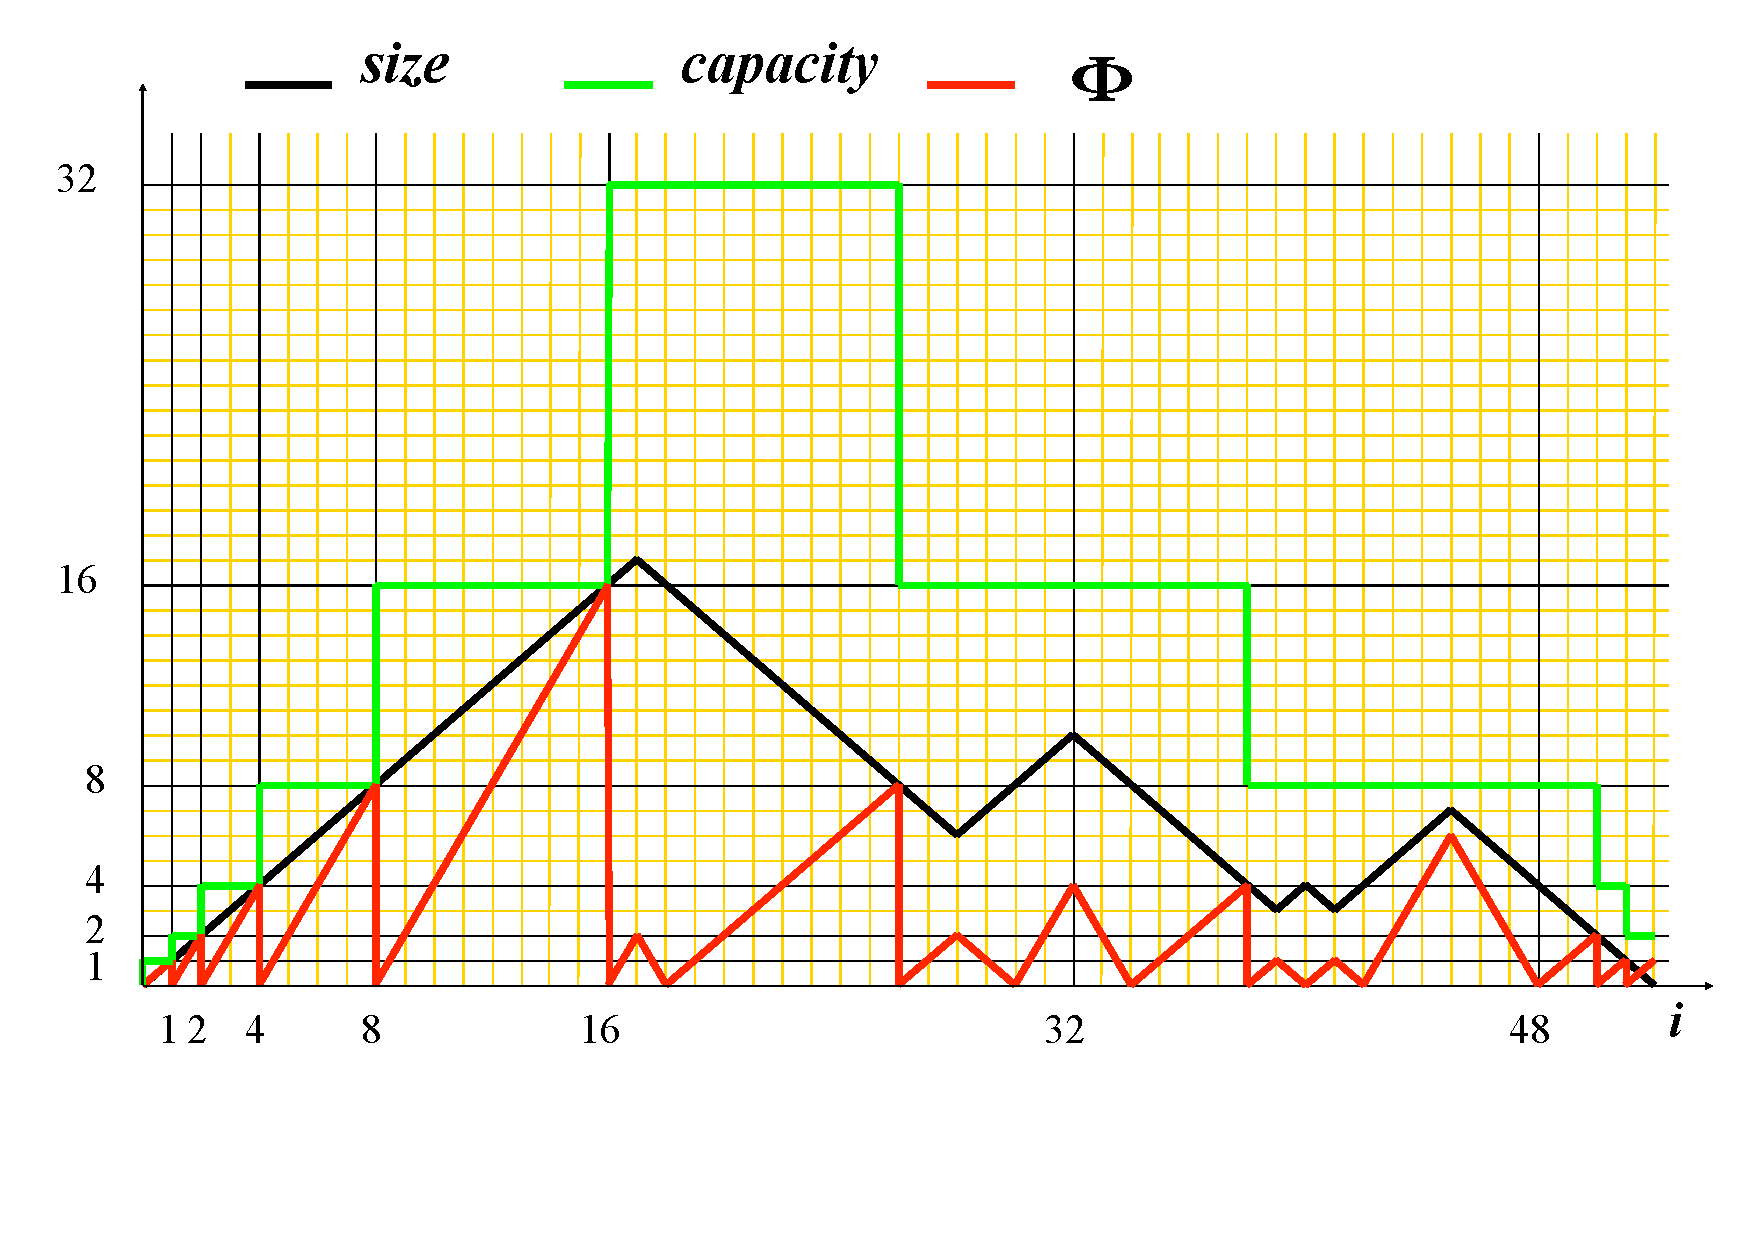
\includegraphics[width=.65\textwidth]{dynvector}
    \caption{Didascalia}\label{fig:dynvector}
\end{figure}

Se \(\alpha=\frac{1}{2}\) il costo ammortizzato di un inserimento \emph{senza espansione} è:
\[\begin{WithArrows}[displaystyle]
a_i &= c_i + \Phi_i - \Phi_{i-1} \Arrow{sostituisco}\\
    &= 1 + (2 \cdot \text{dim}_i - \text{capacità}_i) - (2 \cdot \text{dim}_{i-1} - \text{capacità}_{i-1}) \Arrow{sostituisco}\\
    &= 1 + 2 \cdot (\text{dim}_{i-1}) - \text{capacità}_{i-1} - 2 \cdot \text{dim}_{i-1} + \text{capacità}_{i-1} \Arrow{sostituisco}\\
    &= 3
\end{WithArrows}\]

Se \(\alpha=1\) il costo ammortizzato di un inserimento \emph{con espansione} è:
\[\begin{WithArrows}[displaystyle]
a_i &= c_i + \Phi_i - \Phi_{i-1} \Arrow{sostituisco}\\
    &= 1 + \text{dim}_{i-1} + (2 \cdot \text{dim}_i - \text{capacità}_i) - (2 \cdot \text{dim}_{i-1} - \text{capacità}_{i-1}) \Arrow{sostituisco}\\
    &= 1 + \text{dim}_{i-1} + 2 \cdot (\text{dim}_{i-1}) - \text{capacità}_{i-1} - 2 \cdot \text{dim}_{i-1} + \text{capacità}_{i-1} \Arrow{sostituisco}\\
    &= 3
\end{WithArrows}\]

\paragraph{Esercizio}
Calcola altri casi per valori differenti di \(\alpha\) e per contrazione.

\subsection{Conclusioni}

Esempi di applicazione dell'analisi ammortizzata sono l'espansione e la contrazione di tabelle hash, insiemi disgiunti con euristica sul rango e compressione dei cammini, Heap di Fibonacci.

\subsubsection{Ristrutturazione di tabelle Hash}

Nella ristrutturazione di tabelle hash non è conveniente che \(\alpha\) cresca troppo, in particolare con la scansione interna.
Ma vale anche per le liste di trabocco.

Sopra la soglia \(t_{\alpha}\) prefissata (tipicamente \(0.5\)-\(0.75\)), si alloca una nuova tabella di dimensione \(2m\) e si reinseriscono tutte le chiavi presenti nella nuova tabella.
Il risultato è che il fatto di carico è dimezzato (tipicamente \(0.25\)) e che nessun elemento risulta \enquote{\textbf{deleted}}.

I costi per la ristrutturazione nel caso pessimo è \(\Omicron(m)\).
Il costo ammortizzato è costante (vedi la dimostrazione per i vettori).

\begin{table}[!hb]\centering
    \caption{Reality check}
    \begin{tabular}{@{} *{4}{l} @{}}
        \toprule
            \textbf{Linguaggio} & \textbf{Tecnica} & \(t_{\alpha}\) & \textbf{Note}\\
        \midrule
            Java 7 \texttt{HashMap} & Liste di trabocco basate su \texttt{LinkedList} & \(0.75\) & \makecell[l]{\(\Omicron(n)\) nel caso pessimo\\Overhead: \(16n + 4m\) byte}\\
        \lightrule
            Java 8 \texttt{HashMap} & Liste di trabocco basate su RB Tree & \(0.75\) & \makecell[l]{\(\log n\) nel caso pessimo\\Overhead: \(48n + 4m\) byte}\\
        \lightrule
            C++ \texttt{sparse\_hash} & Ind. aperto, scansione quadratica & ? & Overhead: \(2n\) bit\\
        \lightrule
            C++ \texttt{dense\_hash} & Ind. aperto, scansione quadratica & \(0.5\) & \makecell[l]{\(X\) byte per chiave-valore\\\(\rightarrow\) 2-3\(X\) overhead}\\
        \lightrule
            C++ \texttt{unordered\_map} & Liste di trabocco basate su liste & \(1.00\) & MurmurHash\\
        \lightrule
            Python & Indirizzam. aperto, scansione quadratica & \(0.66\) &\\
        \bottomrule
    \end{tabular}
\end{table}

\ifsubfile
\end{document}
\fi